\section{La retropropagación}
\begin{figure}[H]
	\centering
    \scalebox{0.8}{\input{img/retro}}
    \caption{Algoritmo de retropropagación}
\end{figure}

\section{El gradiente descendente}% http://alejandrosanchezyali.blogspot.cl/2016/01/algoritmo-del-gradiente-descendente-y.html
El gradiente descendente busca los punto $p \in \Omega$ donde funciones del tipo $f: \Omega\subseteq\mathbb{R}^m \rightarrow \mathbb{R}$ alcanzan su mínimo. La idea de este método se basa en que si $f$ es una función diferenciable en todo su dominio $\Omega$, entonces la derivada de $f$ es un punto $p \in \Omega$ en dirección de un vector unitario $v \in \mathbb{R}^m$ se define como

$$ df_{p}(v) = \nabla f(p)v $$

Observe que la magnitud de la ecuación es
$$ |d f_{p}(v)| = ||\nabla f(p)|| ||v||\cos\theta = ||\nabla f(p)\cos\theta$$

Dicha magnitud es máxima cuando $\theta = 2n\pi, n \in \mathbb{Z}$. Es decir, para que $|df_{d}(v)|$ sea máxima, los vectores $\nabla f(p)$ y $v$ debe ser paralelo. De esta manera, la función $f$ crece más rápidamente en la dirección del vector $\nabla f(p)$ y decrece más rápidamente en la dirección del vectro $-\nabla f(p)$. Dicha situación sugiere que la dirección negativa del gradiente $-\nabla f(p)$ es una buena dirección de búsqueda para encontrar el minimizador de la función $f$.

Sea $f: \Omega \subseteq \mathbb{R} \rightarrow \mathbb{R}$, si $f$ tiene un mínimo en $p$, para encontrar a $p$ se construye una sucesión de punto $\{p_{t}\}$ tal que $p_{t}$ converge a $p$. Para resolver esto, comenzamos en $p_{t}$ y nos desplazamos una cantidad $-\lambda_{t}\nabla f(p_{t})$ para encontrar el punto $p_{t + 1}$ más cercano a $p$, es decir:
$$ p_{t + 1} =p_{t} - \lambda _{t}\nabla f(p_{t}) $$

donde $\lambda_{t}$ se selecciona de tal manera que $p_{t + 1} \in \Omega$ y $f(p_{t}) \geq f(p_{t + 1})$

El parámetro $\lambda_{t}$ se seleccionara para maximizar la cantidad a la que decrece la función $f$ en cada paso.


\begin{figure}[H]
	\centering
    \scalebox{0.6}{% http://staff.itee.uq.edu.au/janetw/cmc/chapters/BackProp/index2.html
% http://outlace.com/Beginner-Tutorial-Backpropagation/
% http://neuralnetworksanddeeplearning.com/chap2.html
% http://staff.itee.uq.edu.au/janetw/cmc/chapters/BackProp/slides/Backprop_files/frame.htm
% http://staff.itee.uq.edu.au/janetw/cmc/chapters/BackProp/
% http://home.agh.edu.pl/~vlsi/AI/backp_t_en/backprop.html
% https://www.google.cl/webhp?sourceid=chrome-instant&ion=1&espv=2&ie=UTF-8#safe=off&q=backpropagation+practice+example
% https://ayearofai.com/rohan-4-the-vanishing-gradient-problem-ec68f76ffb9b#.9ntv81akz

\ifx\du\undefined
  \newlength{\du}
\fi
\newcommand{\nweigth}[2]{$W^{#1}_{#2} - \alpha\frac{\partial J}{\partial W^{#1}_{#2}}$}
\newcommand{\w}[2]{$W^{#1}_{#2}$}

\setlength{\du}{1\unitlength}
\begin{tikzpicture}[font=\small]
\tikzstyle{neuron}=[circle,draw, minimum size=2em]
\tikzstyle{update}=[dashed, blue]

\pgftransformxscale{1.000000}
\pgftransformyscale{-1.000000}

\coordinate (x1)    at (0.000000\du, 0.000000\du);
\coordinate (x2)    at (0.000000\du, 8.000000\du);

\coordinate (i)     at (3.000000\du, 0.000000\du);
\coordinate (ii)    at (3.000000\du, 8.000000\du);

\coordinate (iv)    at (10.000000\du, 0.000000\du);
\coordinate (v)     at (10.000000\du, 8.000000\du);

\coordinate (vii)   at (17.000000\du, 0.000000\du);
\coordinate (viii)  at (17.000000\du, 8.000000\du);

\coordinate (ix)   at (17.000000\du, 0.000000\du);
\coordinate (diez)  at (17.000000\du, 8.000000\du);


\coordinate (x)     at (24.000000\du, 4.000000\du);
\coordinate (y)     at (27.000000\du, 4.000000\du);


%%%%%%%%%%%%%%%%%%%%%%%%%%%%%%%%%%%%%%%%%%%%%%%%%%%%%%%%%%
% ENTRADA
\node (X1) at (x1) {\Huge $x_1$};
\node (X2) at (x2) {\Huge $x_2$};

% CAPA DE ENTRADA
\node[neuron] (A) at  (i) {}; % A
\node[neuron] (B) at  (ii)  {}; % B

% CAPA 1
\node[neuron] (C) at  (iv)  {}; % C
\node[neuron] (D) at  (v)  {}; % D

% CAPA 2
\node[neuron] (E) at  (vii)  {}; % E
\node[neuron] (F) at  (viii)  {}; % F

% CAPA 2
\node[neuron] (H) at  (ix)  {}; % E
\node[neuron] (I) at  (diez)  {}; % F

% CAPA DE SALIDA
\node[neuron] (G) at  (x)  {}; % G

% SALIDA
\node (out) at (y) {\Huge $y_1$};
%%%%%%%%%%%%%%%%%%%%%%%%%%%%%%%%%%%%%%%%%%%%%%%%%%%%%%%%%%


\draw[->] (X1) -- (A);
\draw[->] (X2) -- (B);


%%%%%%%%%%%%%%%%%%%%%%%%%%%%%%%%%%%%%%%%%%%%%%%%%%%%%%%%%%
%%%%%%%%%%%%%%%%%%%%%%%%%%%%%%%%%%%%%%%%%%%%%%%%%%%%%%%%%%
\draw[->] (A) -- node[above, pos=0.2] (W_1_11) {\w{1}{11}} (C);
\draw[->] (A) -- node[left , pos=0.2] (W_1_12) {\w{1}{12}} (D);
\draw[->] (B) -- node[left , pos=0.2] (W_1_13) {\w{1}{13}} (C);
\draw[->] (B) -- node[below, pos=0.2] (W_1_14) {\w{1}{14}} (D);

%\draw[->, dashed, blue] (C) to [bend left=40] node[above] {$W^{1}_{11} - \alpha\frac{\partial J}{\partial W^{1}_{11}}$} (W_1_11);
\draw[->, update] (C) to [bend left=40] node[above] {\nweigth{1}{11}} (W_1_11);
\draw[->, update] (D) to [bend left=50] node[above right, pos=0.98] {\nweigth{1}{12}} (W_1_12);

\draw[->, update] (C) to [bend right=50] node[below right, pos=0.98] {\nweigth{1}{13}} (W_1_13);
\draw[->, update] (D) to [bend right=40] node[below] {\nweigth{1}{14}} (W_1_14);

%%%%%%%%%%%%%%%%%%%%%%%%%%%%%%%%%%%%%%%%%%%%%%%%%%%%%%%%%%
%%%%%%%%%%%%%%%%%%%%%%%%%%%%%%%%%%%%%%%%%%%%%%%%%%%%%%%%%%
\draw[->] (C) -- node[above, pos=0.2] (W_2_11) {\w{l}{11}} (E);
\draw[->] (C) -- node[left , pos=0.2] (W_2_12) {\w{2}{12}} (F);
\draw[->] (D) -- node[left , pos=0.2] (W_2_13) {\w{2}{13}} (E);
\draw[->] (D) -- node[below, pos=0.2] (W_2_14) {\w{2}{14}} (F);

\draw[->, update] (E) to [bend left=40] node[above] {\nweigth{2}{11}} (W_2_11);
\draw[->, update] (F) to [bend left=50] node[above right, pos=0.98] {\nweigth{2}{12}} (W_2_12);

\draw[->, update] (E) to [bend right=50] node[below right, pos=0.98] {\nweigth{2}{13}} (W_2_13);
\draw[->, update] (F) to [bend right=40] node[below] {\nweigth{2}{14}} (W_2_14);

%%%%%%%%%%%%%%%%%%%%%%%%%%%%%%%%%%%%%%%%%%%%%%%%%%%%%%%%%%
%%%%%%%%%%%%%%%%%%%%%%%%%%%%%%%%%%%%%%%%%%%%%%%%%%%%%%%%%%
\draw[->] (E) -- node[right, pos=0.2] (W_3_11) {\w{3}{11}} (G);
\draw[->] (F) -- node[right, pos=0.2] (W_3_12) {\w{3}{12}} (G);

\draw[->, update] (G) to [bend  left=50] node[above right, pos=0.98] {\nweigth{3}{11}} (W_3_11);
\draw[->, update] (G) to [bend right=40] node[below right, pos=0.98] {\nweigth{3}{12}} (W_3_12);


\draw[->] (G) -- (out);
\end{tikzpicture}
}
    \caption{$W^{1}_{ij}$ es el peso de la $n$-ésima neurona en la capa $l - 1$ a la $j$-ésima neurona de la capa $l$ de la red.}
\end{figure}

\section{El problema del gradiente descendente}
El proceso iterativo que implementan los algoritmos de optimización, lentamente se dirigen hacia un óptimo local, perturbando los pesos en una dirección deducida mediante el uso del gradiente, de tal manera que disminuye a la función de costo. El algoritmo de gradiente descendente actualiza los pesos por el negativo del gradiente ponderado por un valor escalar entre 0 y 1.

\begin{algorithm}[H]
	\SetAlgoLined
	\caption{Algoritmo del gradiente descendente}
	\KwData{$C$: La función de costo.}
	\KwResult{Valor óptimo de la función de costo $C$}
	initialization\;
	\While{$\frac{\partial C}{\partial W^{l}_{ij}} \rightarrow 0$}{
		$W^{l}_{ij} = W^{l}_{ij} - \alpha\frac{\partial C}{\partial W^{l}_{ij}}$\;
	}
\end{algorithm}

\newpage
Se busca un algoritmo que permita encontrar pesos y sesgos para que la salida de la red aproxime los valores de $y(x)$ a los valores correspondientes con cada entrada $x$. De esta manera, será posible cuantificar qué tan bien se logra el objetivo mediante la función de costo

$$C(w, b) = \frac{1}{2n}\sum_{x} ||y(x) - a||^2$$

Donde $w$ denota la colección de todos los pesos de la red, $b$ es el sesgo, $n$



\section{El gradiente descendente estocástico}
% http://neuralnetworksanddeeplearning.com/chap1.html
% http://sebastianruder.com/optimizing-gradient-descent/index.html#gradientdescentvariants
El método del gradiente descendente estocástico (SGD) actualiza los parámetros en cada ejemplo $x_i$ y etiquta $y_i$ de la siguiente manera $$ \theta = \theta - \eta\nabla_\theta $$
    %\begin{figure}[H]
    %    \centering
    %    \scalebox{0.6}{% http://home.agh.edu.pl/~vlsi/AI/backp_t_en/backprop.html
%\ifx\du\undefined
%  \newlength{\du}
%\fi
%\newcommand{\nweigth}[2]{$W^{#1}_{#2} - \alpha\frac{\partial J}{\partial W^{#1}_{#2}}$}
%\newcommand{\w}[2]{$W^{#1}_{#2}$}

%\setlength{\du}{15\unitlength}
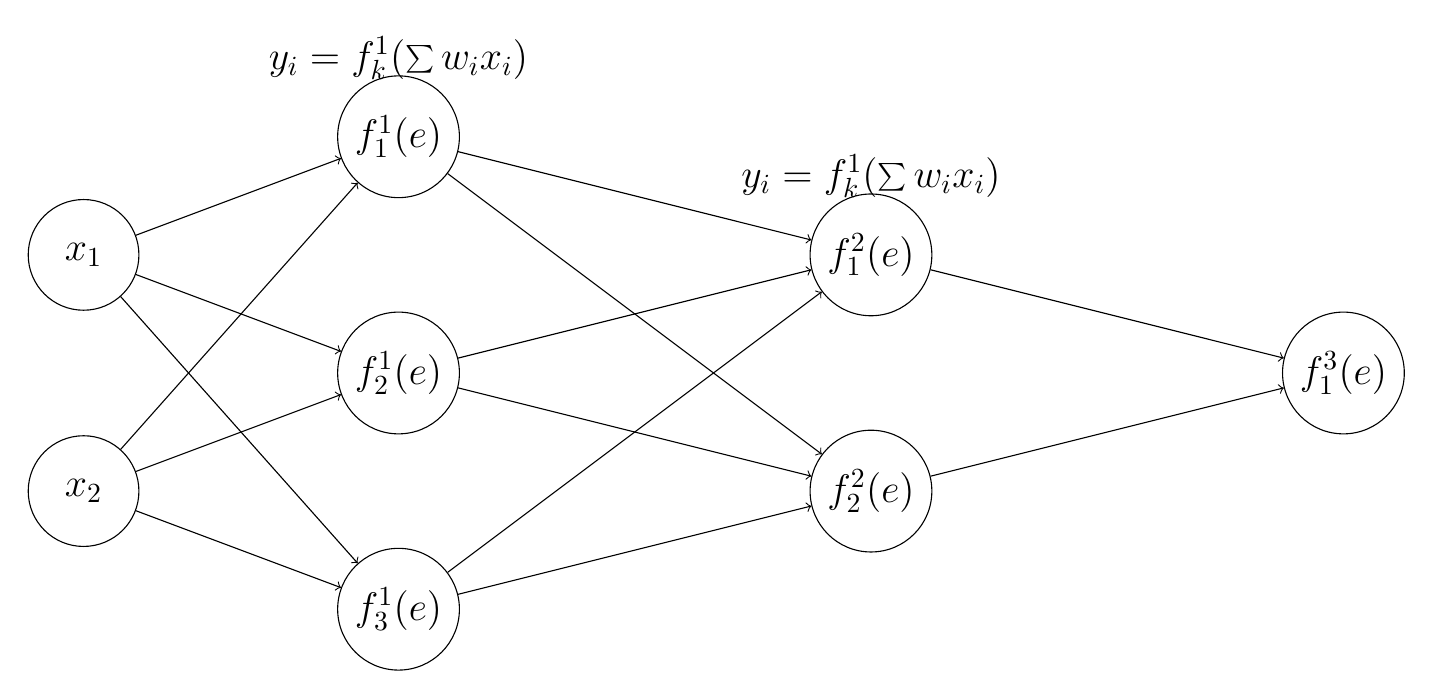
\begin{tikzpicture}
\tikzstyle{neuron}=[circle,draw, minimum size=4em, font=\Large]
\tikzstyle{update}=[dashed, blue]

\coordinate (x_1) at (-5, 1.5);
\coordinate (x_2) at (-5, -1.5);

\coordinate (n_1_1) at (-1, 3);
\coordinate (n_1_2) at (-1, 0);
\coordinate (n_1_3) at (-1, -3);

\coordinate (n_2_1) at (5, 1.5);
\coordinate (n_2_2) at (5, -1.5);

\coordinate (n_3_1) at (11, 0);


\node[neuron] (x_1) at (x_1) {$x_{1}$};
\node[neuron] (x_2) at (x_2) {$x_{2}$};

\node[neuron] (n_1_1) at (n_1_1) {$f^{1}_{1}(e)$};
\node[neuron] (n_1_2) at (n_1_2) {$f^{1}_{2}(e)$};
\node[neuron] (n_1_3) at (n_1_3) {$f^{1}_{3}(e)$};

\node[neuron] (n_2_1) at (n_2_1) {$f^{2}_{1}(e)$};
\node[neuron] (n_2_2) at (n_2_2) {$f^{2}_{2}(e)$};

\node[neuron] (n_3_1) at (n_3_1) {$f^{3}_{1}(e)$};


\node[above of=n_1_1] {\Large $y_i = f^{1}_{k}(\sum w_i x_i)$};
\node[above of=n_2_1] {\Large $y_i = f^{1}_{k}(\sum w_i x_i)$};
%\node[above of=n_3_1] {\Large $y_i = f^{1}_{k}(\sum w_i x_i)$};

\draw[->] (x_1) -- (n_1_1);
\draw[->] (x_1) -- (n_1_2);
\draw[->] (x_1) -- (n_1_3);
\draw[->] (x_2) -- (n_1_1);
\draw[->] (x_2) -- (n_1_2);
\draw[->] (x_2) -- (n_1_3);

\draw[->] (n_1_1) -- (n_2_1);
\draw[->] (n_1_1) -- (n_2_2);
\draw[->] (n_1_2) -- (n_2_1);
\draw[->] (n_1_2) -- (n_2_2);
\draw[->] (n_1_3) -- (n_2_1);
\draw[->] (n_1_3) -- (n_2_2);

\draw[->] (n_2_1) -- (n_3_1);
\draw[->] (n_2_2) -- (n_3_1);

\end{tikzpicture}
}
    %\end{figure}
